% Created 2024-06-26 Wed 18:38
% Intended LaTeX compiler: xelatex
\documentclass[11pt]{article}
\usepackage{hyperref}
% TIPS
% \substack{a\\b} for multiple lines text





% pdfplots will load xolor automatically without option
\usepackage[dvipsnames]{xcolor}

\usepackage{forest}
% two-line text in node by [two \\ lines]
% \begin{forest} qtree, [..] \end{forest}
\forestset{
  qtree/.style={
    baseline,
    for tree={
      parent anchor=south,
      child anchor=north,
      align=center,
      inner sep=1pt,
    }}}
%\usepackage{flexisym}
% load order of mathtools and mathabx, otherwise conflict overbrace

\usepackage{mathtools}
%\usepackage{fourier}
\usepackage{pgfplots}
\usepackage{amsthm, mathabx,  amsmath, commath}
\usepackage{amsfonts}

\usepackage{empheq}
\usepackage{tikz}
\usetikzlibrary{arrows.meta}
\usepackage[most]{tcolorbox}

\newtheorem{theorem}{Theorem}[section]
\newtheorem{definition}{Definition}[section]
\newtheorem{corollary}{Corollary}[section]
\newtheorem{example}{Example}[section]
\newtheorem{lemma}{Lemma}[section]
\newtheorem{proposition}{Proposition}[section]

\newcommand{\bl}[1] {\boldsymbol{#1}}
\newcommand{\Wt}[1] {\stackrel{\sim}{\smash{#1}\rule{0pt}{1.1ex}}}
\newcommand{\wt}[1] {\widetilde{#1}}


%For boxed texts in align, use Aboxed{}
%otherwise use boxed{}

\DeclareMathSymbol{\widehatsym}{\mathord}{largesymbols}{"62}
\newcommand\lowerwidehatsym{%
  \text{\smash{\raisebox{-1.3ex}{%
    $\widehatsym$}}}}
\newcommand\fixwidehat[1]{%
  \mathchoice
    {\accentset{\displaystyle\lowerwidehatsym}{#1}}
    {\accentset{\textstyle\lowerwidehatsym}{#1}}
    {\accentset{\scriptstyle\lowerwidehatsym}{#1}}
    {\accentset{\scriptscriptstyle\lowerwidehatsym}{#1}}
}

\usepackage{graphicx}
    
% text on arrow for xRightarrow
\makeatletter
%\newcommand{\xRightarrow}[2][]{\ext@arrow 0359\Rightarrowfill@{#1}{#2}}
\makeatother


\def \bx {\boldsymbol{x}}
\def \ba {\boldsymbol{a}}
\def \bI {\boldsymbol{I}}
\def \bt {\boldsymbol{t}}
\def \bb {\boldsymbol{b}}
\def \bA {\boldsymbol{A}}
\def \bX {\boldsymbol{X}}
\def \bu {\boldsymbol{u}}
\def \bS {\boldsymbol{S}}
\def \bZ {\boldsymbol{Z}}
\def \bz {\boldsymbol{z}}
\def \by {\boldsymbol{y}}
\def \bw {\boldsymbol{w}}
\def \bT {\boldsymbol{T}}
\def \bS {\boldsymbol{S}}
\def \bm {\boldsymbol{m}}
\def \bW {\boldsymbol{W}}
\def \bY {\boldsymbol{Y}}
\def \bH {\boldsymbol{H}}
\def \blambda {\boldsymbol{\lambda}}
\def \bPhi {\boldsymbol{\Phi}}
\def \btheta {\boldsymbol{\theta}}
\def \bmu {\boldsymbol{\mu}}
\def \bphi {\boldsymbol{\phi}}
\def \bSigma {\boldsymbol{\Sigma}}
\def \lb {\left\{}
\def \rb {\right\}}
\def \caln {\mathcal{N}}
\def \dissum {\displaystyle\Sigma}
\def \dispro {\displaystyle\prod}
\def \E {\mathbb{E}}
\def \Q {\mathbb{Q}}
\def \V {\mathbb{V}}
\def \R {\mathbb{R}}
\def \calq {\mathcal{Q}}
\def \calg {\mathcal{G}}
\def \caln {\mathcal{N}}
\def \calr {\mathcal{R}}
\def \calm {\mathcal{M}}
\def \calc {\mathcal{C}}
\def \bcup {\bigcup}

\graphicspath{{../../books/}}
\makeindex

%% ox-latex features:
%   !announce-start, !guess-pollyglossia, !guess-babel, !guess-inputenc, caption,
%   image, !announce-end.

\usepackage{capt-of}

\usepackage{graphicx}

%% end ox-latex features


\author{Nancy Lynch}
\date{\today}
\title{Distributed Algorithms}
\hypersetup{
 pdfauthor={Nancy Lynch},
 pdftitle={Distributed Algorithms},
 pdfkeywords={},
 pdfsubject={},
 pdfcreator={Emacs 29.1 (Org mode 9.8-pre)}, 
 pdflang={English}}
\begin{document}

\maketitle
\tableofcontents

\section{Mutual Exclusion}
\label{sec:orgd2ea250}

\subsection{Asynchronous Shared Memory Model}
\label{sec:org16414bd}
The system is modelled as a collection of processes and shared variables,
with interactions. Each process \(i\) is a kind of state machine, with a set statesi of states and a subset \(start\) of \(states_i\) indicating the
start states, just as in the synchronous setting. However, now process \(i\) also has labelled
\(actions\), describing the activities in which it participates. These are classified as either
\(input\), \(output\), or \(internal\) actions. We further distinguish between two different kinds of
internal actions: those that involve the shared memory and those that involve strictly local
computation. If an action involves the shared memory, we assumethat it only involves one shared
variable.

There is a transition relation \(trans\) for the entire system, which is a set of \((s,\pi,s')\)
triples, where and \(s'\) are \textbf{automaton states}, that is, combinations of states for all the
processes and values for all the shared variables, and where \(\pi\)  is the label of an input,
output, or internal action. We call these combinations of process states and variable values
``automaton states'' because  the entire system is modelled as a single automaton. The statement that
\((s,\pi,s')\in trans\) says that from automaton state \(s\) it is possible to go to automaton state
\(s'\) as a result of performing action \(\pi\).

We assume that input actions can always happen, that is, that the system is input-enabled. Formally,
this means that for every automaton state \(s\) and input action \(\pi\), there exists \(s'\) such
that \((s,\pi,s')\in trans\). In contrast, output and internal steps might be enabled only in a subset
of the states. The intuition behind the input-enabling property is that the input actions are
controlled by an arbitrary external user, while the internal and output actions are controlled by the
system itself.
\subsection{The Problem}
\label{sec:org90fefda}
The mutual exclusion problem involves the allocation of a single, indivisible, nonshareable resource
among \(n\) \textbf{users}, \(U_1,\dots,U_n\).

A user with access to the resource is modelled as being in a \textbf{critical region}, which is simply a
designated subset of its states. When a user is not involved in any way with the resource, it is said
to be in the \textbf{remainder region}. In order to gain admittance to its critical region, a user executes a
\textbf{trying protocol}, and after it is done with the resource, it executes an (often trivial) \textbf{exit protocol}.
This procedure can be repeated, so that each user follows a cycle, moving from its
\emph{remainder region} (R) to its \emph{trying region} (T), then to its \emph{critical region} (C), then to its \emph{exit
region} (E), and then back again to its remainder region.  

\begin{center}
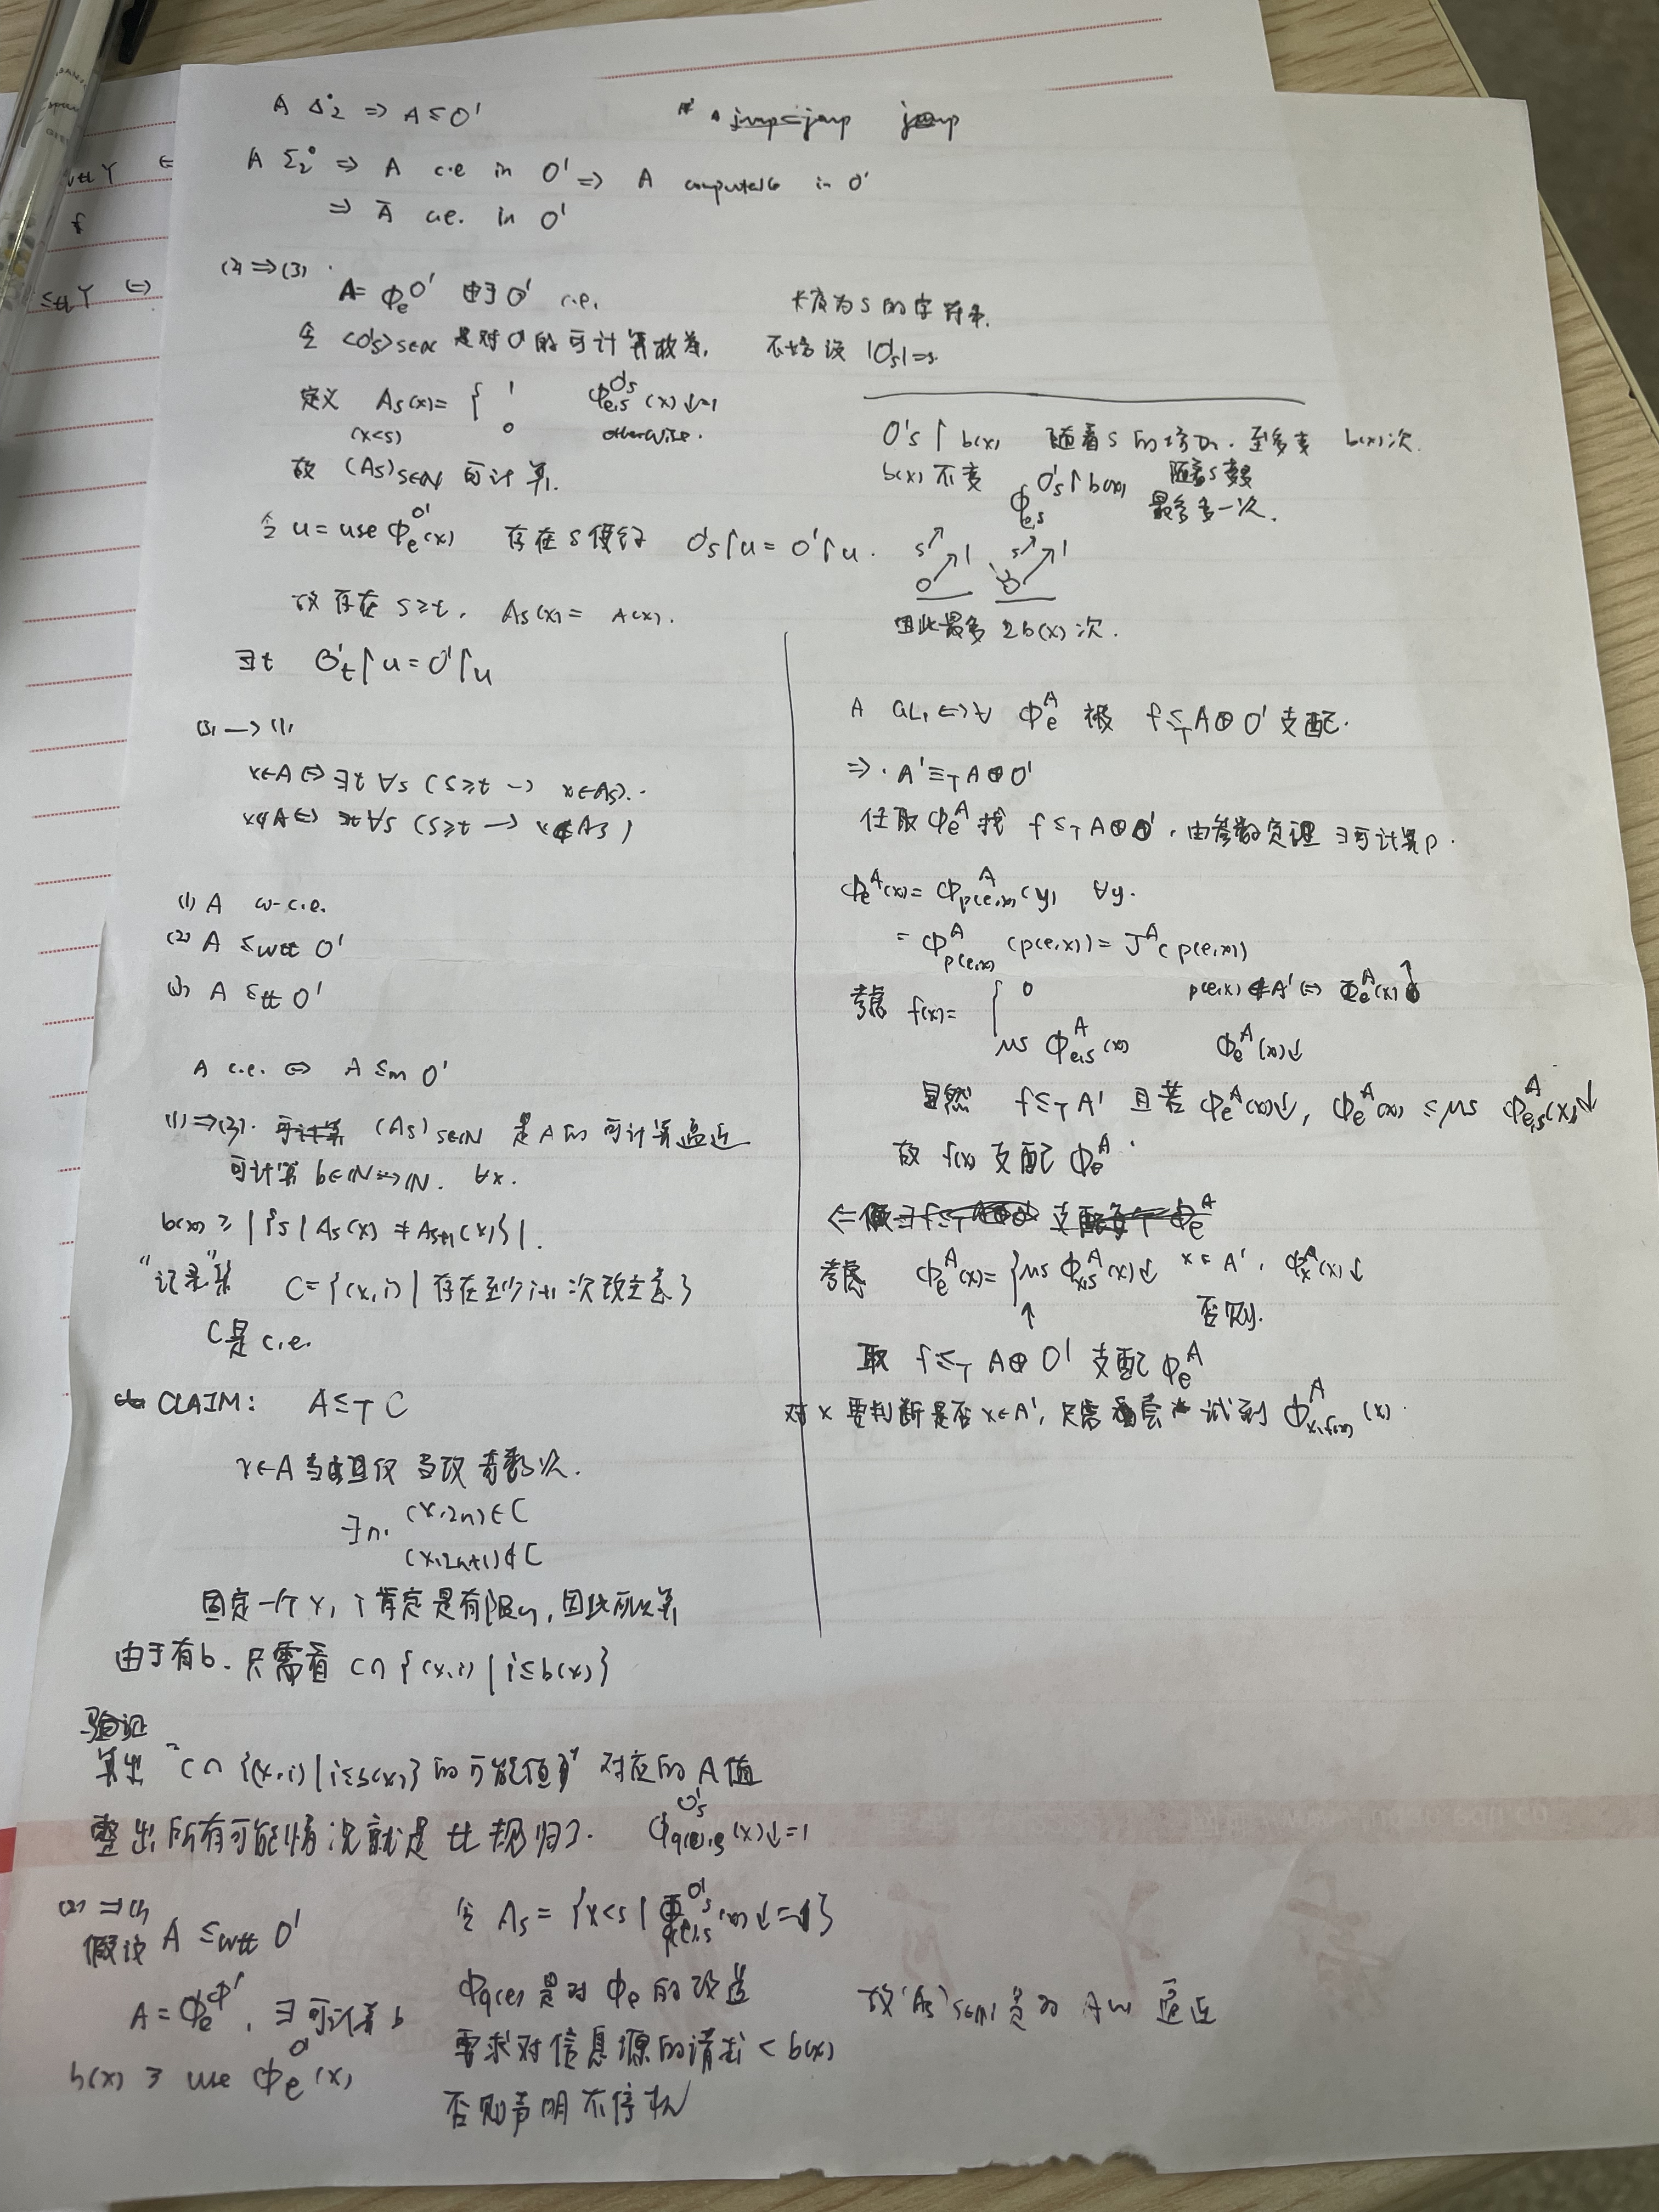
\includegraphics[width=.2\textwidth]{../images/DistributedAlgorithms/1.png}
\captionof{figure}{\label{10.2}The cycle of regions of a single user}
\end{center}

Each 
\end{document}
